\subsection{Introduction}
The goal of this first part is to implement a minimal working simulation of a QAM communication.
In order to achieve that, the up- and downsampling blocks, the RRC filtering blocks and the baseband equivalent model of the channel, as represented in figure~\ref{fig:chain} must be implemented.
\begin{figure}[htbp]
\centering

\caption{Block diagram of the communication system [source: Assignment introduction].\label{fig:chain}}
\end{figure}
The modulator and demodulator are supplied with the assignment statement.

\subsection{Halfroot Nyquist filtering}
After its modulation, the message is upsampled and filtered with a root raised cosine filter to limit its bandwidth occupation.
The effect on the PSD of the signal is shown in figure~\ref{fig:LPF}.
\begin{figure}[htbp]
\centering
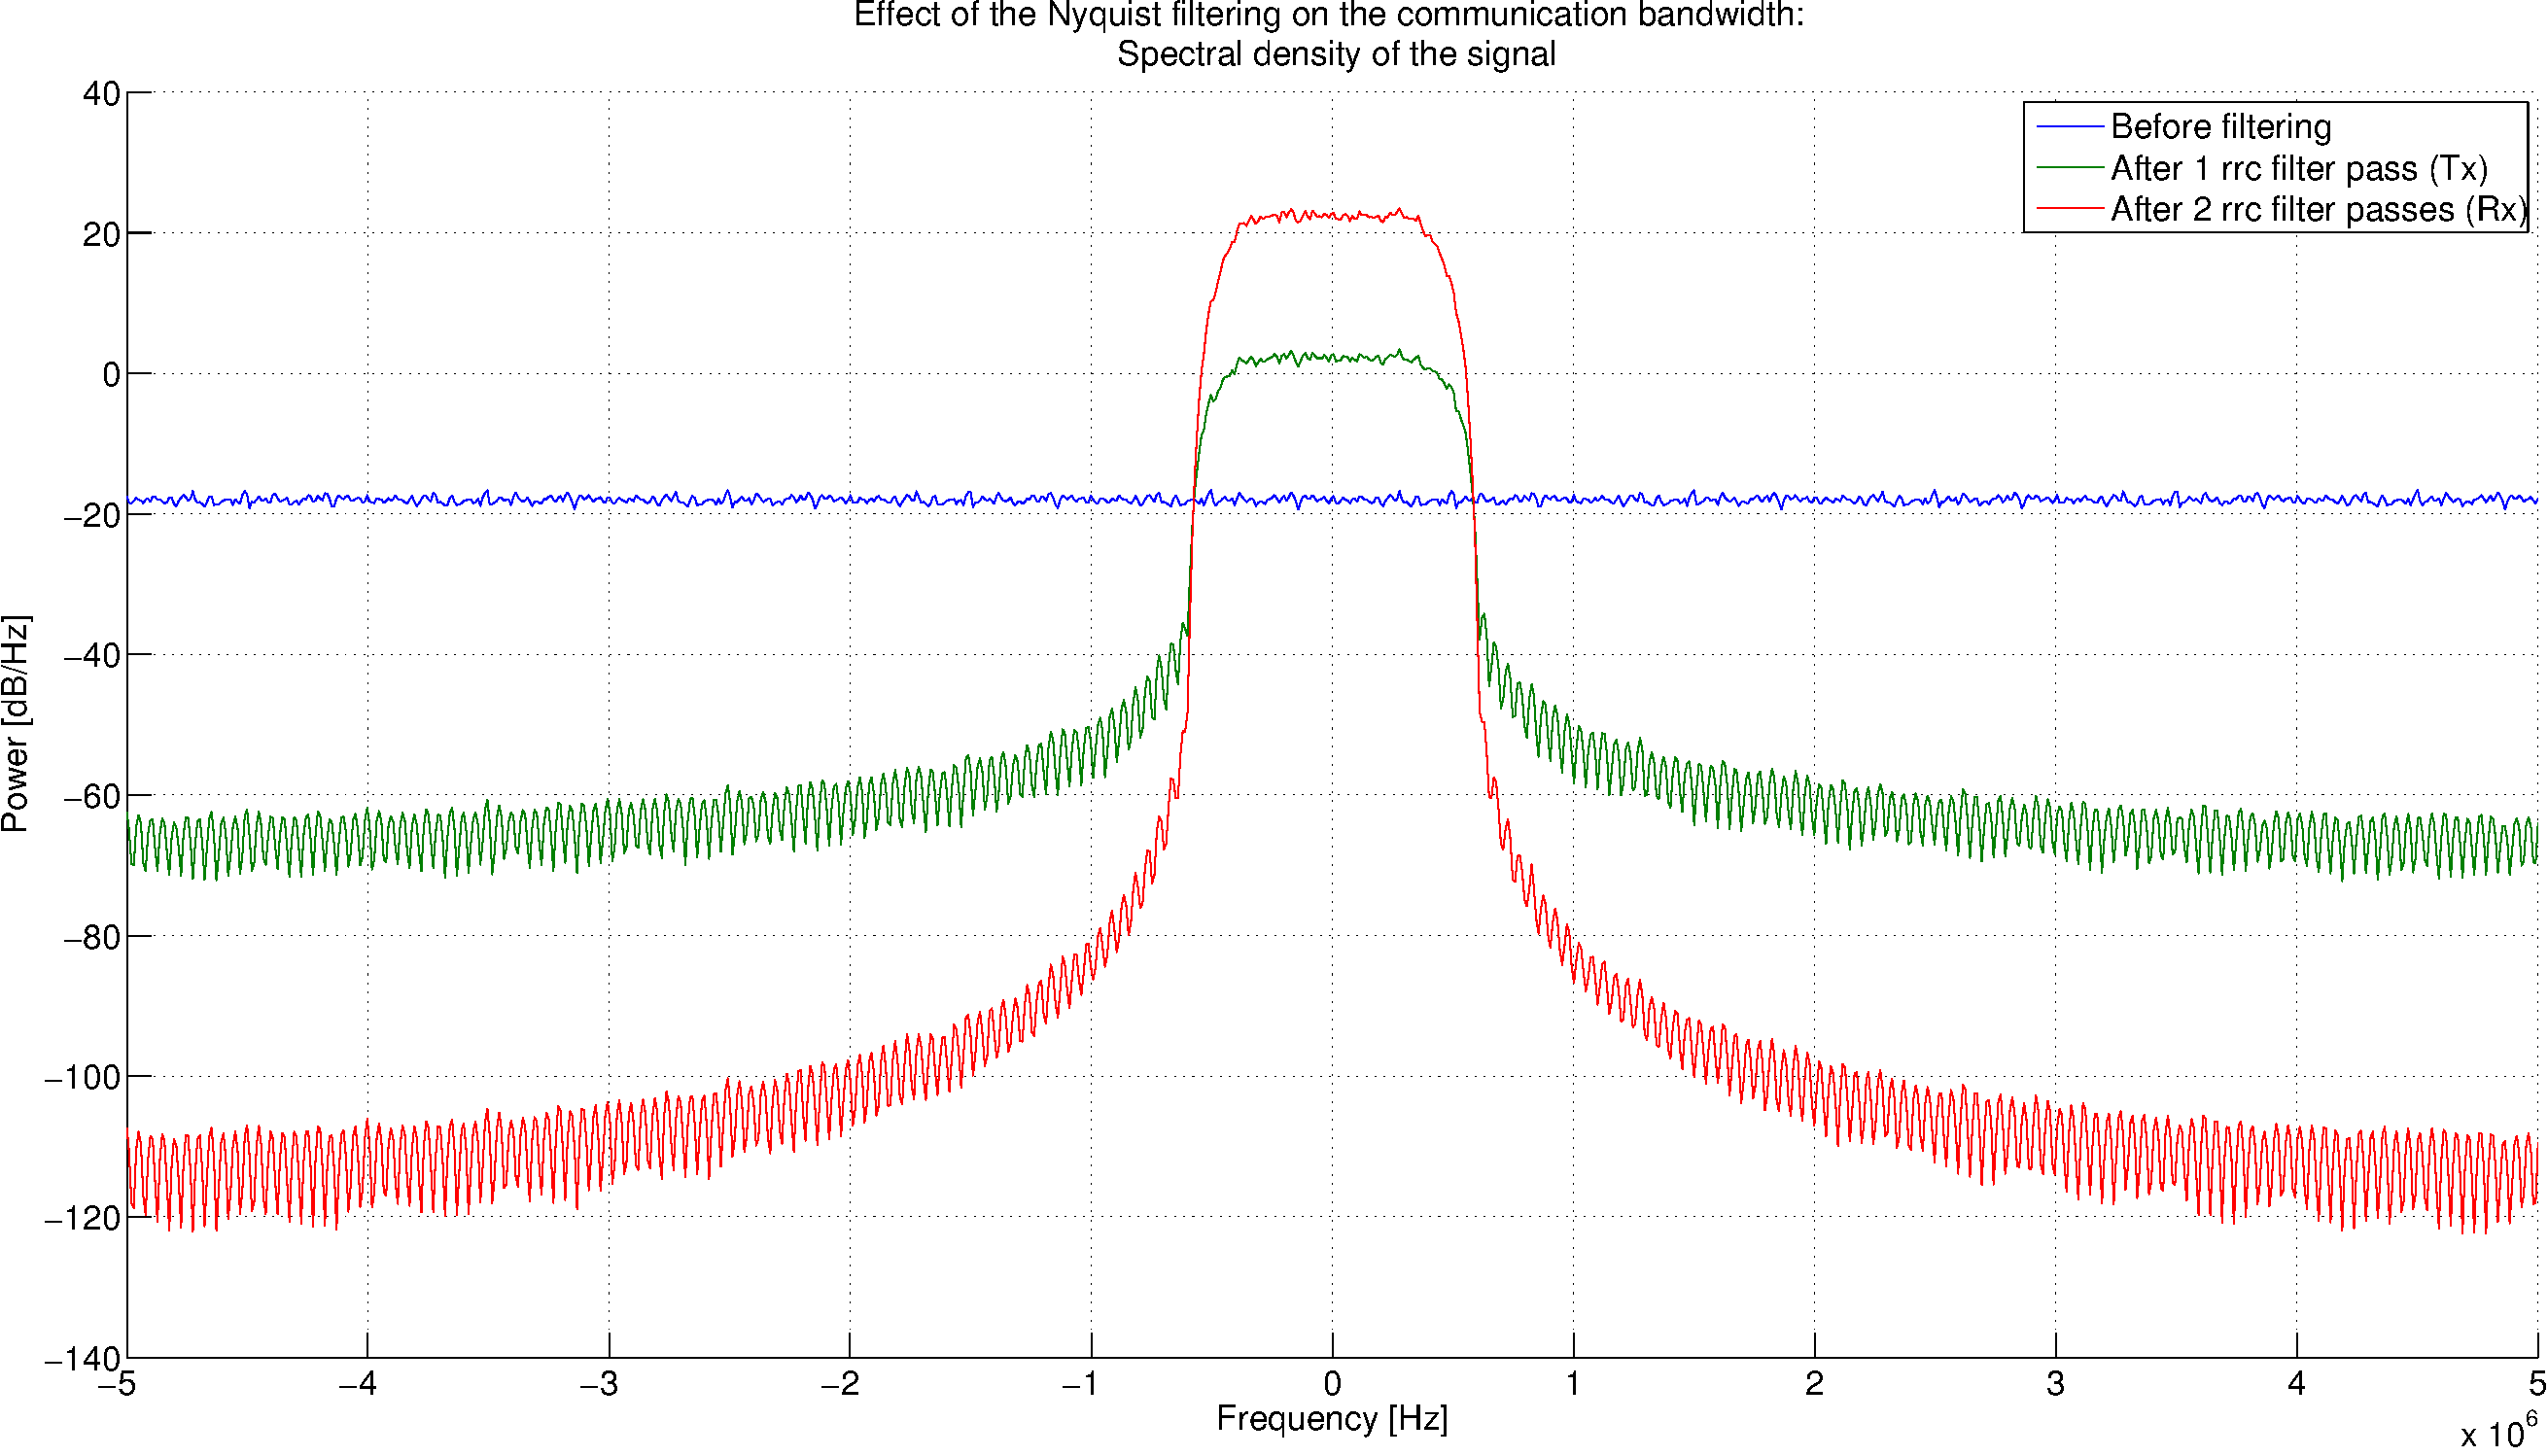
\includegraphics[width=\textwidth]{commBW.pdf}
\caption{Nyquist filtering limits the communication bandwidth.\label{fig:LPF}}
\end{figure}

In order to maximize the SNR at the output, the low pass filtering is split between the transmitter and the receiver.
The halfroot nyquist filter $g(t)$ is such that the resulting operation $h(t) = g(t)*g(t)$ forms a nyquist filter which does not introduce inter symbol interference, as shown in figure~\ref{fig:noISI}
\begin{figure}
\centering
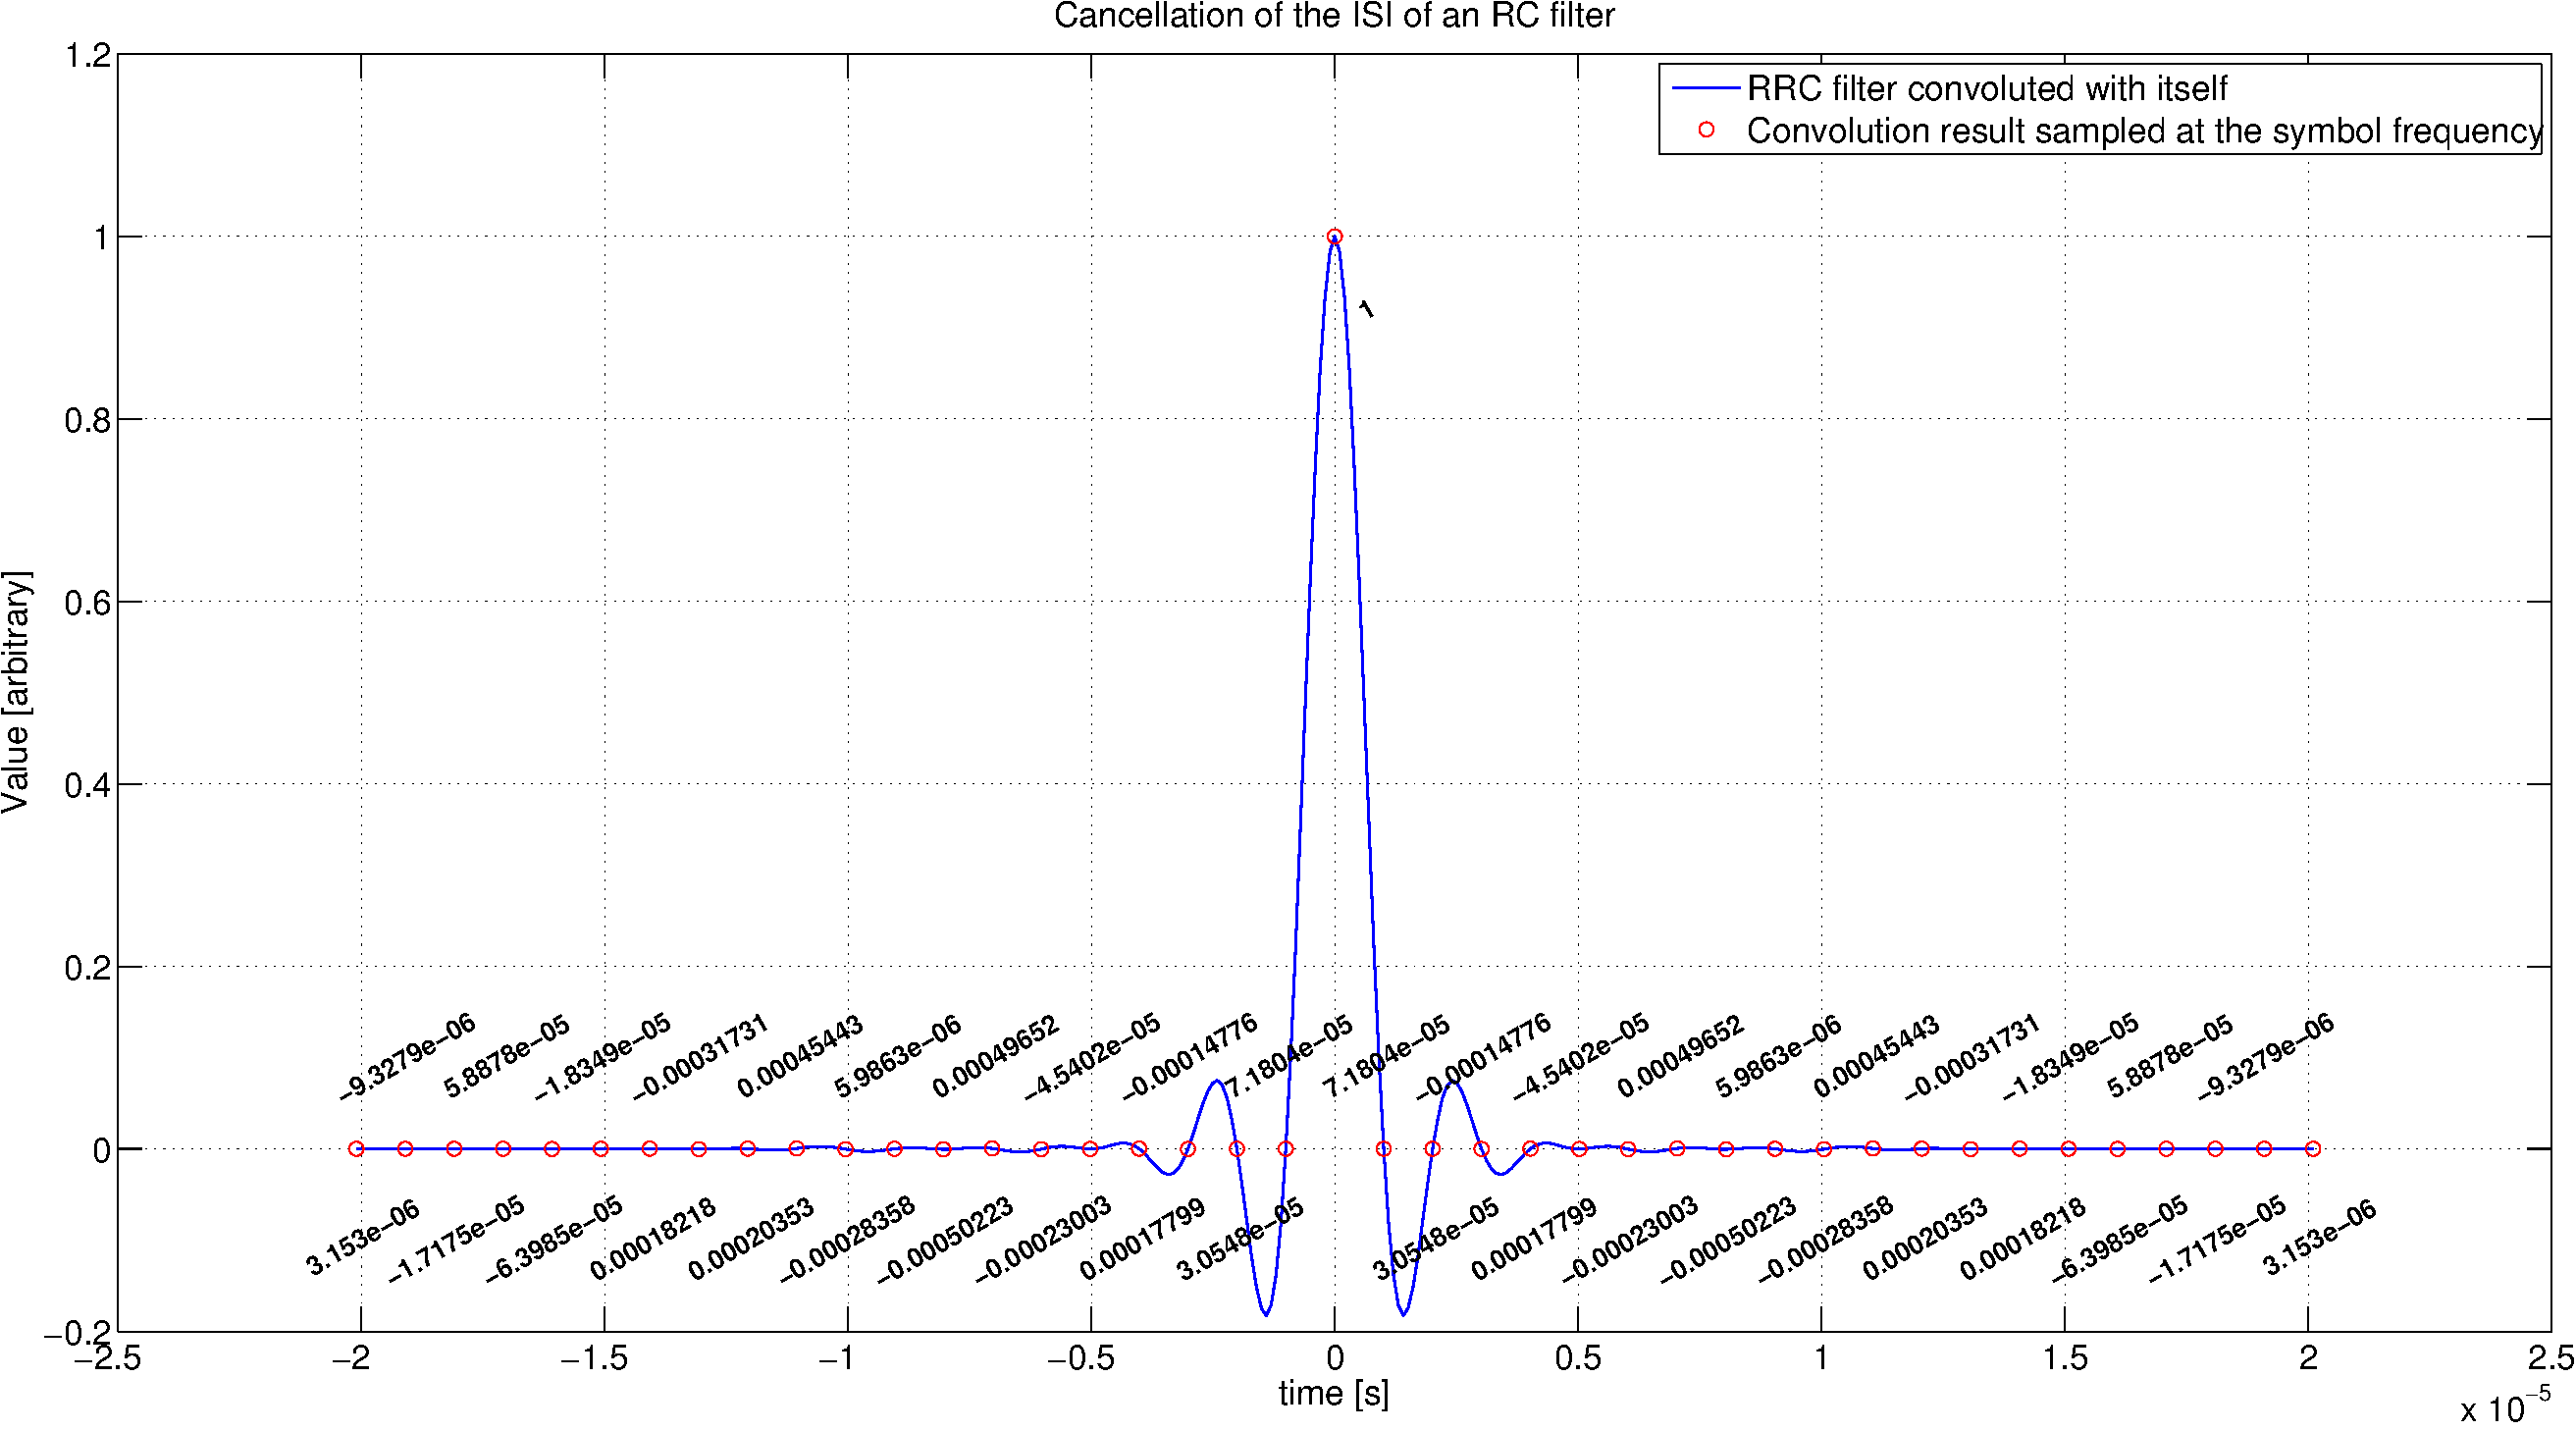
\includegraphics[width = \textwidth]{isi.pdf}
\caption{Cancellation of the inter symbol interference of a raised cosine filter.\label{fig:noISI}}
\end{figure}

\subsection{Impact of the noisy channel}
Theory shows that a channel affected by AWGN can be modelled in the baseband by AWGN of corresponding power.
This allows to easily simulate the BER of the noisy channel.
The results of the simulations are summarized by the BER curves of figure~\ref{fig:BER}
\begin{figure}[htbp]
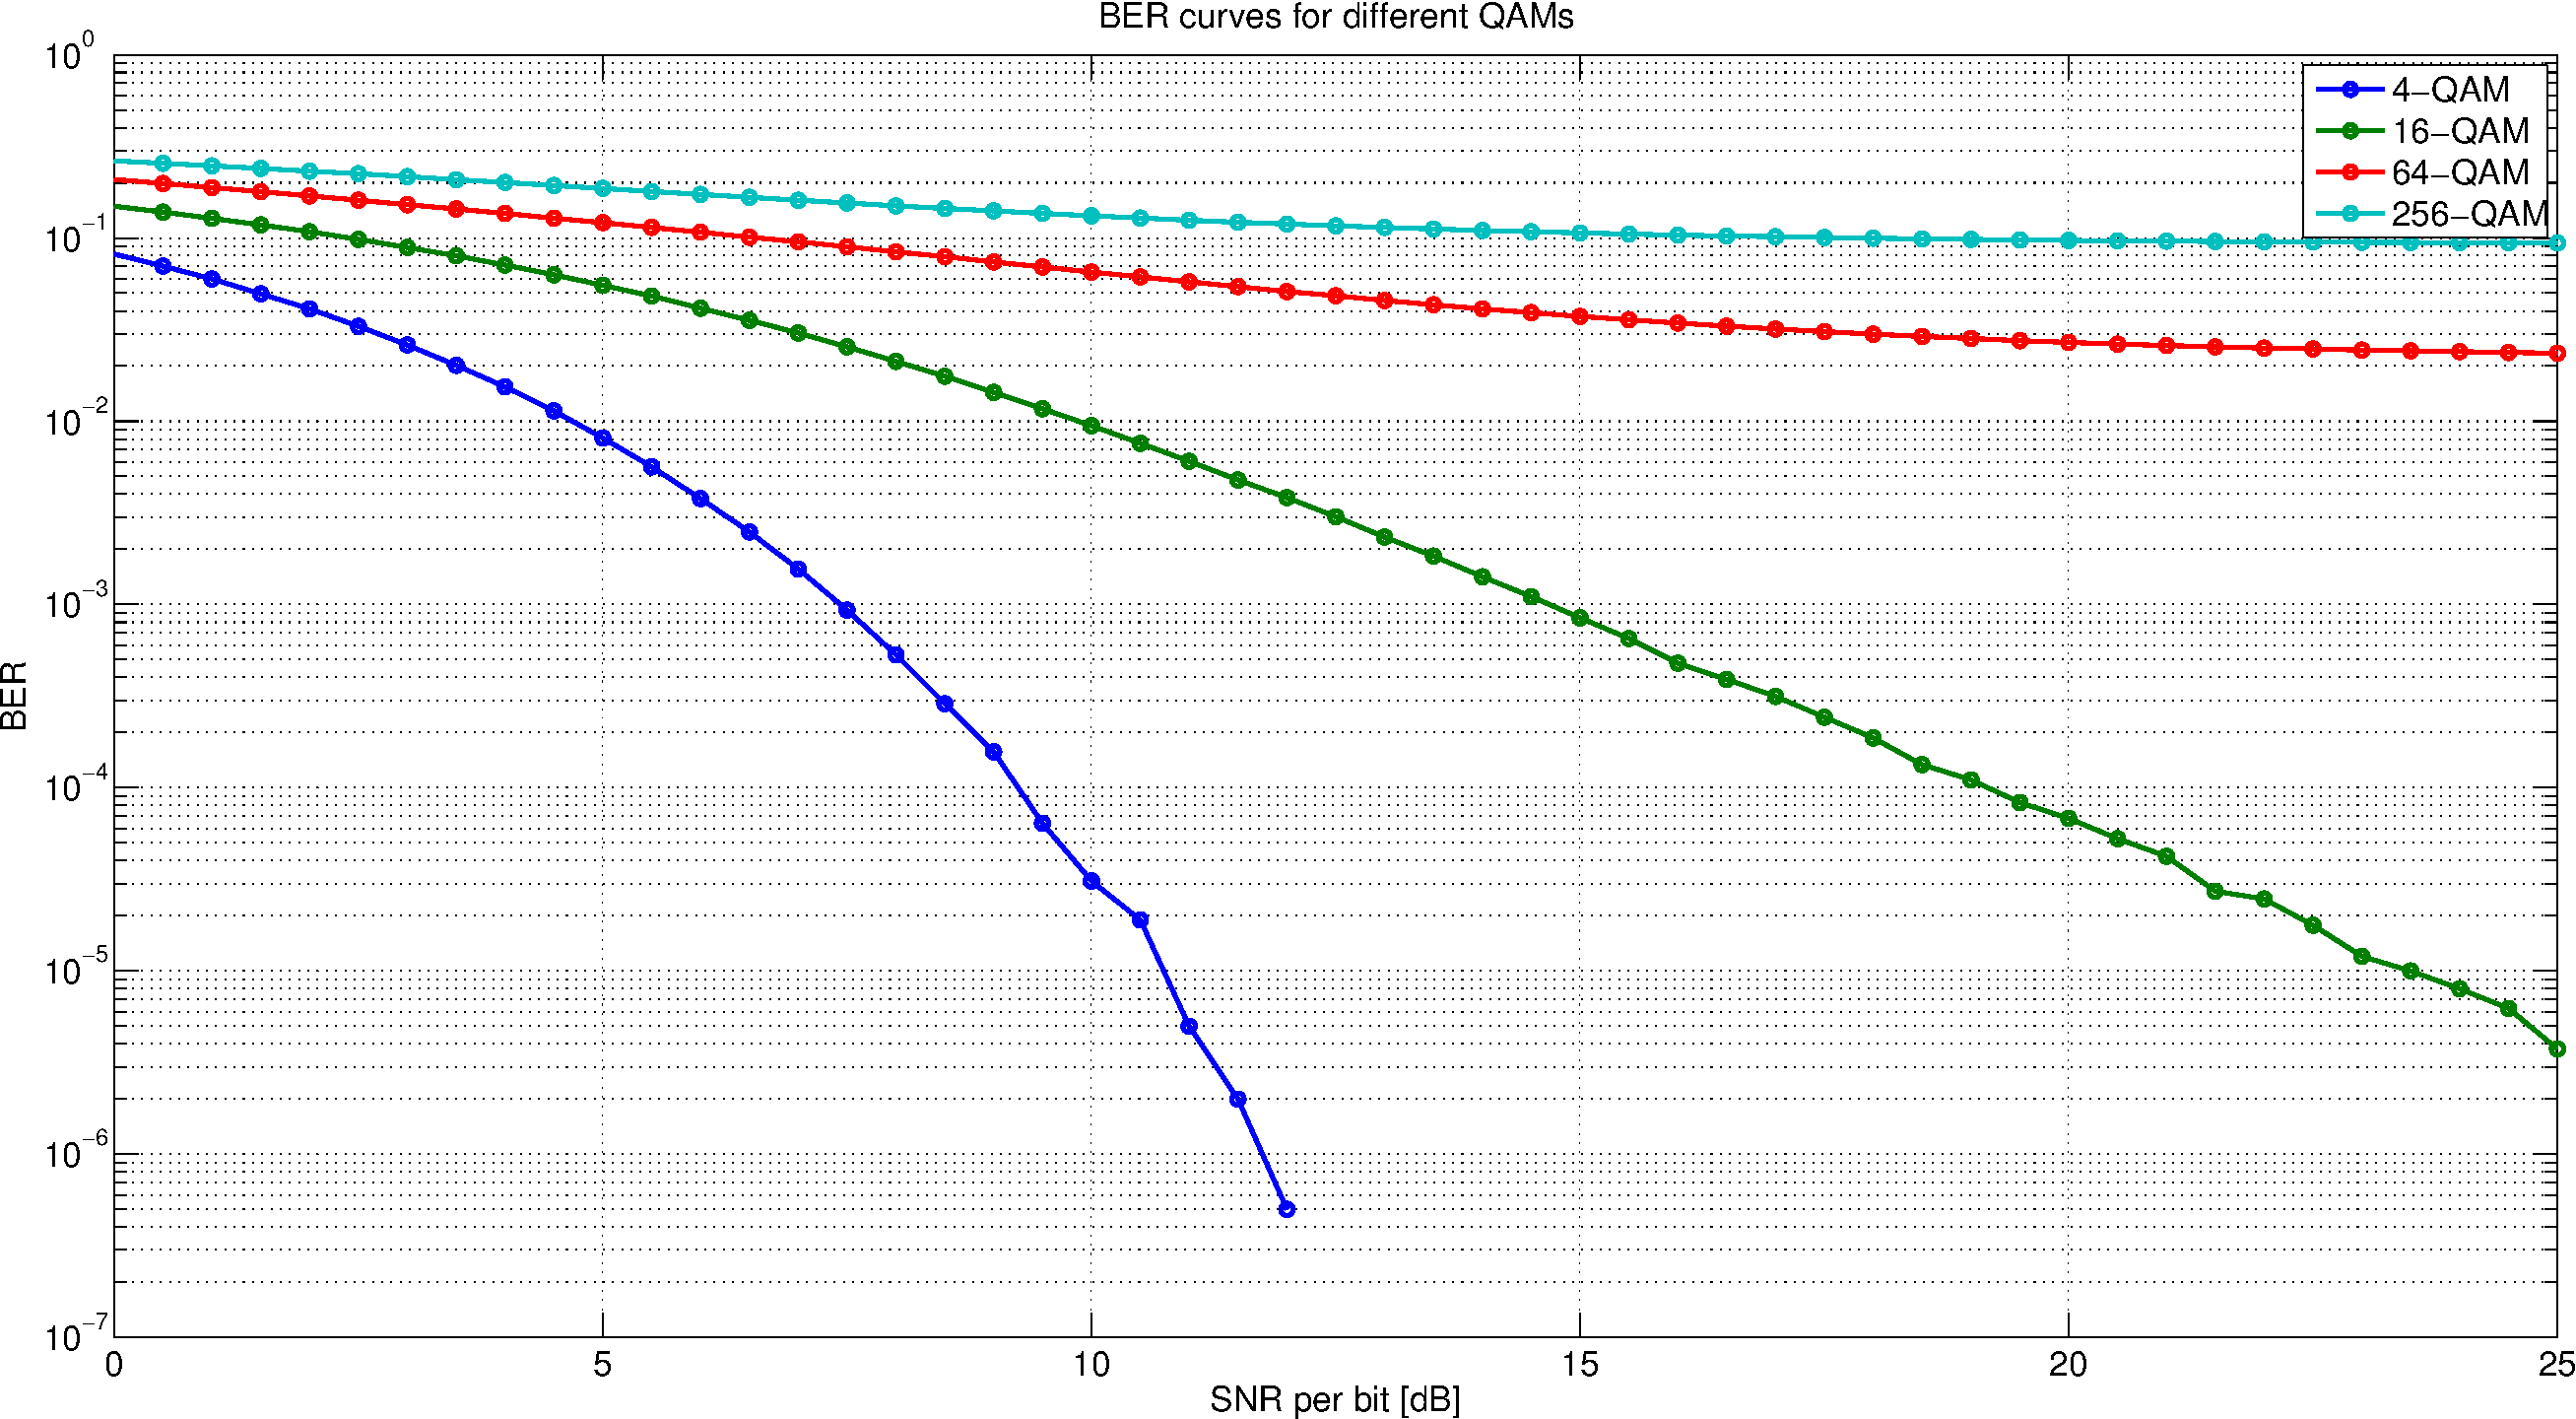
\includegraphics[width=\textwidth]{BERs.pdf}
\caption{BER in function of $\frac{E_b}{N_0}$ for different QAM modulations.\label{fig:BER}}
\end{figure}

\subsection{Questions}
\subsubsection{Simulation}
\paragraph{It is proposed to use the baseband equivalent model of the AWGN channel. Would it be
possible to live with a bandpass implementation of the system?}
The baseband signals have the advantages to first reduce the needed sampling frequency and second it allows to implement modulation and demodulation techniques regardless of the carrier frequency. That is why baseband equivalent is always preferred in modelling wireless communication channels.
\paragraph{How do you choose the sample rate in Matlab?} 
By first being sure the sample rate is at least 2 times greater than the maximal frequency (...?)
\paragraph{How do you make sure you simulate the desired $\frac{E_b}{N_0}$ ratio?}
From the noise, we can compute $N_0$ and compare.
\paragraph{How do you choose the number of transmitted data packets and their length?}
We use a huge number to get reliable results.
\subsubsection{Communication System}
\paragraph{Determine the supported (uncoded) bit rate as a function of the physical bandwidth.} On the internet : R = Bw * log2(1+SNR) (I only found in the course : R = log2(M)/T with R = bit rate, M = number of symbols and T = symbol duration)
\paragraph{Explain the trade-off communication capacity/reliability achieved by varying the constellation size.} 
By increasing the constellation size, it reduces the distance between the constellations so even for the reliability of the communication. (...)
\paragraph{Why do we choose the halfroot Nyquist filter to shape the complex symbols?}
It is used to limit the bandwidth of the signal before transmission and the second halfroot Nyquist matched filter maximizes the SNR. (??)
\paragraph{How do we implement the optimal demodulator? Give the optimisation criterion.}
\paragraph{How do we implement the optimal detector? Give the optimisation criterion.}